\section{MindSqualls}\label{mindsqualls}
\mindsqualls er et .NET bibliotek til LEGOs NXT robotter.
\mindsqualls tillader kommunikation med NXT enheder via. Bluetooth og USB og fungerer ved at sende og modtager beskeder over disse to teknologier.
Biblioteket er skrevet i \csharp og kan dermed anvendes af alle de .NET kompatible sprog.

I det følgende afsnit gives en beskrivelse af bibliotekets struktur samt eksempler på anvendelse.

\paragraph{Abstraktion}
For at gøre det nemt at arbejde med NXT motorer og sensorer er der i \mindsqualls lavet en abstraktion over disse.
Hver type I/O er således implementeret i hver sin klasse med passende funktioner.
Figur \ref{mindsqualls:structure} viser et klassediagram, der beskriver relationerne mellem de primære klasser i \mindsqualls biblioteket.
Herunder gives en kort gennemgang af de primære klasser i \mindsqualls.

\begin{figure}
\centering
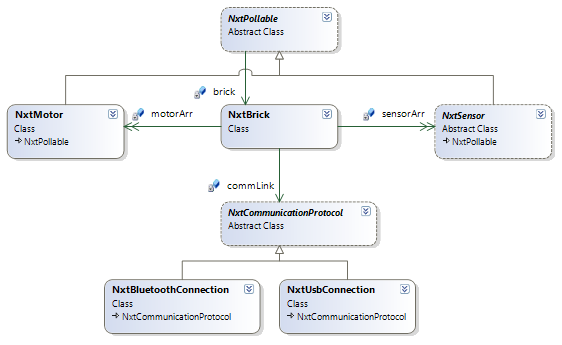
\includegraphics[width=0.8\textwidth]{mindsqualls}
\caption{Den overordnede \mindsqualls struktur}
\label{mindsqualls:structure}
\end{figure}

\subsection{NXT kommunikation}
\mindsqualls opretter forbindelse til NXT enheden vha. klassen \lstinline[style=csharp]!NxtCommunicationProtocol!.
Klassen fungerer, som navnet indikerer, som en protokol ved at definere en række abstrakte funktioner;
Der kan oprettes forbindelse til NXT enheden.
Denne kan afbrydes igen, og det kan til enhver tid fastslås om der er forbindelse til enheden.
Selve kommunikationen sker via kald til funktionen \lstinline[style=csharp]!Send! der tager et array af bytes som input og giver et array af bytes som output.
Altså kan funktionen både sende og modtage beskeder til og fra enheden.
Ved at lave specialiseringer af \lstinline[style=csharp]!NxtCommunicationProtocol! klassen, der definere disse funktioner, kan der kommunikeres med NXT enheden.
Der findes i \mindsqualls to specialiseringer af protokollen;
\begin{itemize}
\item \lstinline[style=csharp]!NxtUsbConnection!\\
Tillader kommunikation via USB (kablet)
\item \lstinline[style=csharp]!NxtBluetoothConnection!\\
Tillader kommunikation via Bluetooth (trådløst)
\end{itemize}

\subsection{Input og Output}
For hver af de sensorer og motorer \lego producerer findes der i \mindsqualls en tilsvarende sensor.
Disse arver alle fra klassen \lstinline[style=csharp]!NxtPollable! der definerer metoder til at læse værdier fra de forskellige komponenter.
Dette gøres ved et \emph{Poll} der opdaterer den enkelte klasses tilstand således at den svarer til det fysiske komponent.
Samtidig er der for \lstinline[style=csharp]!NxtPollable! implementeret parallel automatisk polling.
Altså er det muligt automatisk at opdatere et komponents status.
Brugen af polling (både manuel og automatisk) kan ses i \lstref{mindsqualls:polling}.

Som et eksempel på brugen af sensor-klasser betragtes \legos ultralyds sensor (figur \ref{sensor:ultrasonic_sensor}), som er repræsenteret ved klassen \lstinline[style=csharp]!NxtUltrasonicSensor!.
Denne har en property \lstinline[style=csharp]!DistanceCm! der, som navnet angiver, returnerer afstanden fra sensoren til væggen.

\begin{lstlisting}[style=csharp,caption={Et eksempel på polling i \mindsqualls},label=mindsqualls:polling]
NxtUltrasonicSensor sensor = new NxtUltrasonicSensor();
sensor.OnPolled += pollable =>
    Console.WriteLine("Distance: {0}", sensor.DistanceCm);

sensor.Poll();
// eller
sensor.PollInterval = 100;
\end{lstlisting}